% ---------------------------------------------------------------------------- %
\begin{figure}
	\centering
	\subfigure[\label{fig:linguometer:technical:interference:isd:1}]
	{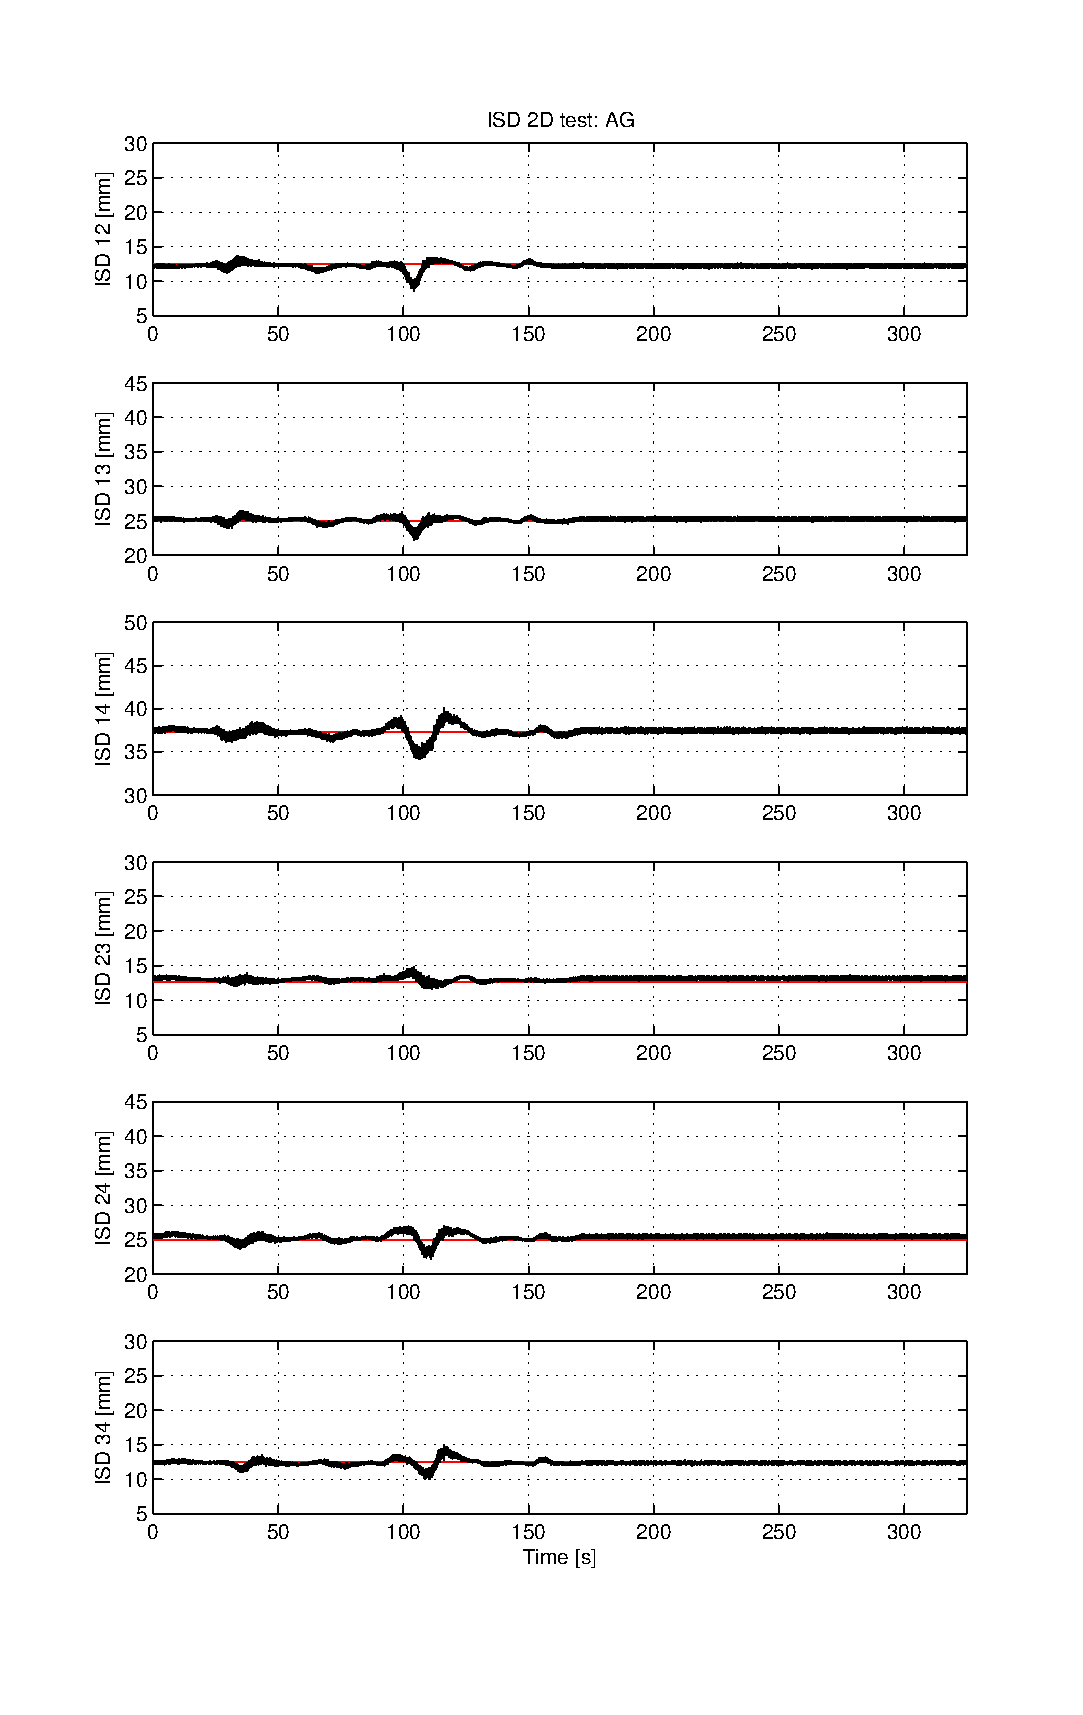
\includegraphics[width=0.35\textwidth]{include/linguometer/images/int_isd3d_1.eps}}
	\subfigure[\label{fig:linguometer:technical:interference:isd:2}]
	{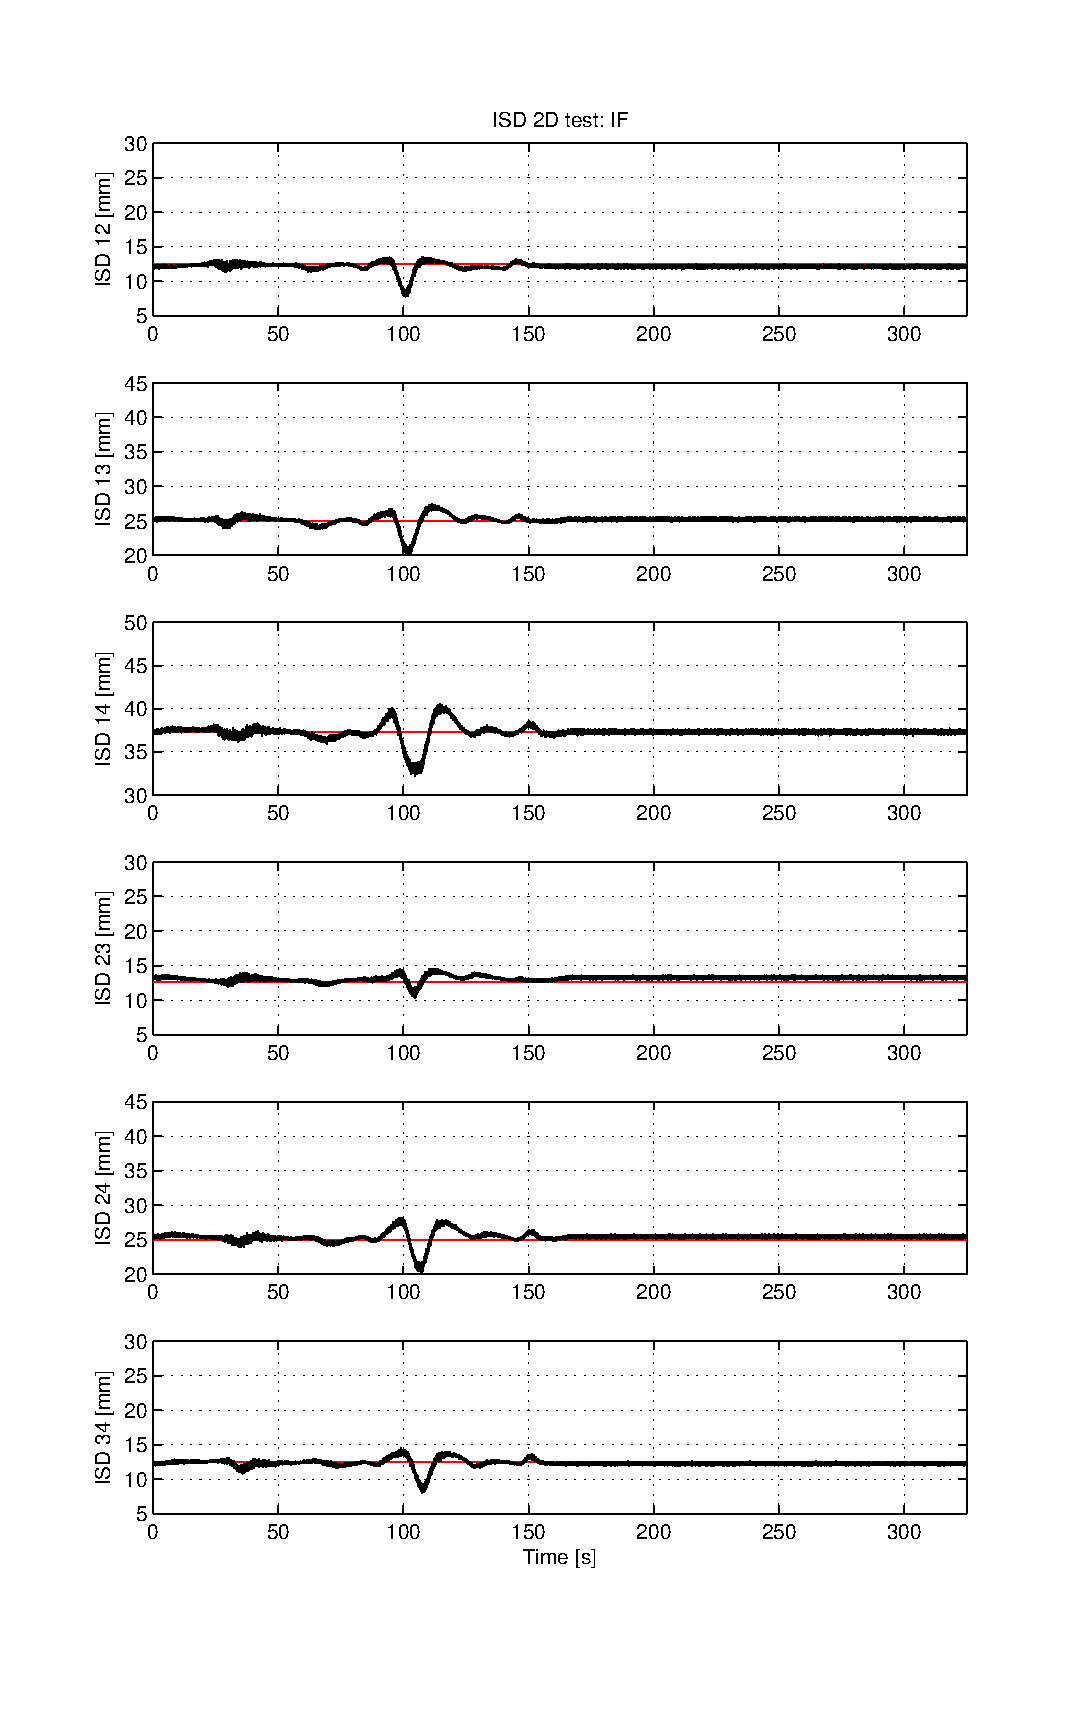
\includegraphics[width=0.35\textwidth]{include/linguometer/images/int_isd3d_2.eps}}

	\subfigure[\label{fig:linguometer:technical:interference:isd:3}]
	{\includegraphics[width=0.35\textwidth]{include/linguometer/images/int_isd3d_3.eps}}
	\hspace{0.35\textwidth}

	\caption[ISD results (ad-hoc test, XYZ)]{\textbf{ISD results (ad-hoc test, XYZ)}:
	ISDs calculated considering the three Cartesian coordinates of each 
	acquired sample (X, Y and Z).
	(a) AG test, (b) IF test and (c) LM test.
	Red plots: ISD between sensors 1 and 2. Black plots: ISD between sensors 2
	and 3. Blue plots: ISD between sensors 3 and 4. 
	Notes: ISD scale in millimiters, time scale in seconds. The revolution of
	the circal starts between 0 and 1.5 seconds and ends approximately at 170
	seconds. From 170 seconds to the end of the acquisition, the sensors remain
	still in the initial position.
	}
	\label{fig:linguometer:technical:interference:isd}
\end{figure}
% ---------------------------------------------------------------------------- %
